\documentclass[titlepage,a4paper]{article}

\usepackage{cmap}
\usepackage[T1]{fontenc}
\usepackage[utf8]{inputenc}
\usepackage[swedish]{babel}
\usepackage{graphicx}
\usepackage{hyperref} 	 
	
\title{Projekt 2, EIT060 Datasäkerhet}

\author{Emil Persson, 920522-2772, dat11epe\\
Valdemar Roxling, 921119-1334, dat11vro}

\begin{document}

\maketitle

\tableofcontents

\newpage

\section{Introduktion}
 Detta projekt är utvecklingen av ett klient-server program som ska hantera känsliga uppgifter, och har därför höga krav på säkerheten. Syftet med utvecklingen är att ge oss mer förståelse för och kunskap om datasäkerhet och SSL. Ett sjukhus har journaler som endast får läsas av berörda patienter, doktorer, sköterskor och Socialstyrelsen. De ska vara åtkomliga men oläsliga för utomstående.

\section{System \& Design}
Systemet består utav en tunn klient vars syfte är att kunna logga in användaren, fastställa en säker anslutning till servern och sedan skicka kommandon och ta emot serverns svar. När klienten distribueras till en användare så skapas ett unikt certifikat för denne användare. Certifikat är illustrerat med en nyckel i figur\ref{design}. Detta certifikat är låst med ett lösenord som används för att senare verifiera användaren vid inloggning. När certifikatet skapas så signeras det av en betrodd certifikatutfärdare, i figur\ref{design} namngiven CA. Denna signering är vital för att anslutningen till serven skall godkännas och tillgång till säkert material ges.
\begin{figure}[!h]
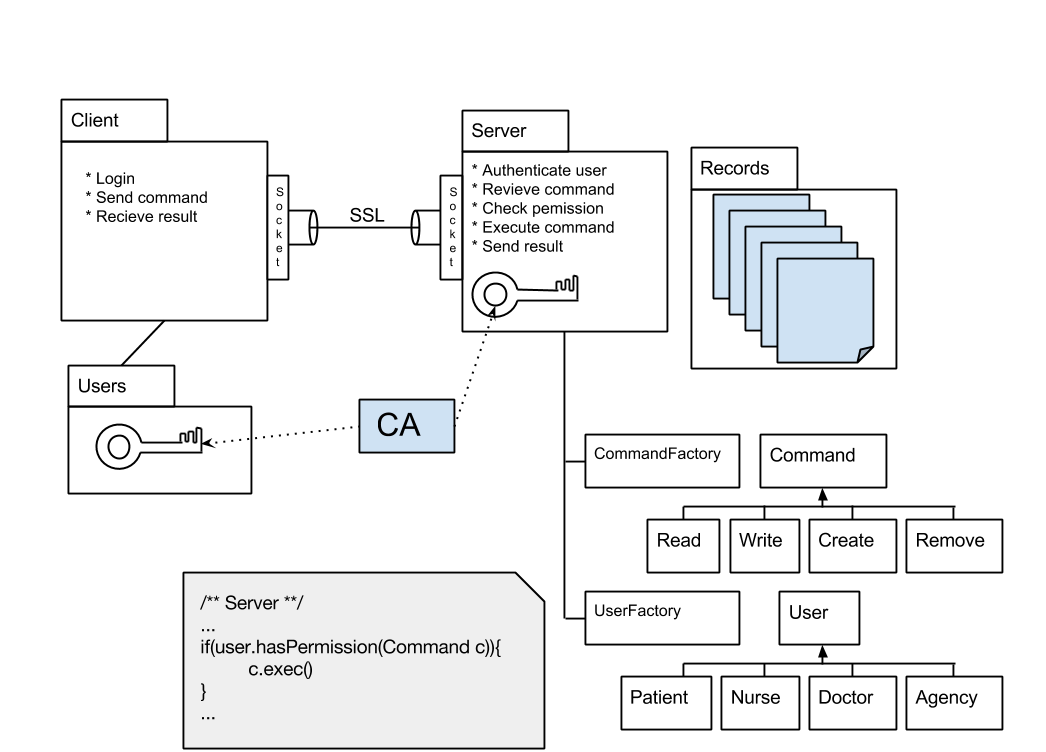
\includegraphics[width=\textwidth]{Design.png}
\caption{Systemdesign}
\label{design}
\end{figure}
Anslutning mellan klienten och servern är av typen SSL “Secure Socket Layer” som är en säker och krypterad anslutning. SSL kräver en att båda parter av anslutningen har var sitt signerat certifikat av samma samma certifikatsutfärdare. Certifikatet i sin tur består utav två nycklar, en privat och en publik. Den publika nyckeln används för att kryptera data som ska skickas och den privata nyckeln används för att dekryptera data som mottagits. Kravet på att certifikaten ska vara signerade av samma certifikatsutfärdare betyder att ingen som inte kan få ett signerat certifikat kommer åt systemet.

När anslutningen är klar används clientens certifikat för att skapa en temporär användare med precis de rättigheter som certifikatet utfärdades för. När sedan ett kommando inkommer från klienten evalueras det och om det motsvarar ett korrekt kommando så kontrolleras om användaren har rättighet att utföra detta kommando innan det utförs, se kodillustration i figur\ref{design}. På så vis garanteras att användare enbart kan utföra kommandon som de har certifierats att utföra. Servern ger feedback på kommandoanrop genom att svara med ett meddelande generarat av kommandot, om det kunde genomföras och i så fall resultatet, annars vilken typ av fel som uppstod.
\newline
\newline
En användare kan vara en utav följande:
\begin{itemize}
\item Patient - En patient har enbart rättighet att läsa sina egna journaler.
\item Nurse - En sjuksköterska har rättighet att läsa och skriva på de patienters journaler som denne är associera med samt läsa alla journaler under samma division.
\item Doctor - En doktor har samma rättigheter som en sjuksköterska men även rättigheter att skapa nya journaler till patienter.
\item Agency - Socialstyrelsen har rättigheter att läsa och ta bort alla journaler i hela systemet.
\end{itemize}

De kommandon som är giltiga är:
\begin{itemize}
\item Create - Skapa en ny journal.
\item Remove -Ta bort en befintlig journal.
\item Read - Läsa en befintlig journal.
\item Write - Skriva till en befintlig journal.
\end{itemize}


\section{Säkerhetsanalys  \& Attacker}
Den huvudsakliga säkerhetsangelägenheten är den möjligheten av olaglig åtkomsten till medicin-journalerna, men det finns även Denial of Service problem. Attackerna på systemer kan ske i 3 områden: på klienten, på servern och på anslutningen.

\begin{itemize}
\item Server
	\begin{description}
	\item [Inbrott] \hfill \\
Servern som journalerna ligger på kan bli stulen, och då har förövarna tillgång till alla filer, medans alla behöriga förlorar tillgång. Vårt projekt ger inget skydd mot ett sådant angrepp, eftersom servern ligger i ett fysiskt skyddat rum, som endast betrodd personal har tillgång till.
	\item [Personal] \hfill \\
Personalen som övervakar servern har full tillgång till alla journaler, och kan via misstag eller medvetet läcka eller sälja filerna till utomstående. De har också rättighet att auktorisera nya klienter, och kan ge ut dem till icke-behöriga. Vårt projekt tillhandahåller ingen lösning till  detta problem, så vi rekommenderar att det krävs legitimation av alla som tar emot en klient, och att den betrodda personalen verkligen är pålitlig.

\item [Malware] \hfill \\
Servern-koden skulle kunna bli modifierad via åtkomsten till klienterna, eller via de två ovanstående punkterna. Vår lösning är skyddad från angrepp via klienter, då endast servern endast tar emot textsträngar ifrån klient. Andra 

	\end{description}
\item Klient

\item Anslutningen
\end{itemize}



\section{Beskrivning av SSL}
nästan slut
\end{document}


